\documentclass{acm_proc_article-sp}

\usepackage{color}
\usepackage{listings}

\definecolor{blue}{rgb}{0.25,0.35,1}
\definecolor{green}{rgb}{0.15,0.8,0.15}
\lstset{
language=sql,
frame=single,
xleftmargin=0.15cm,
morecomment=[l]{@},
commentstyle=\color{green},  
basicstyle=\ttfamily\scriptsize\singlespacing,
keywordstyle=\color{blue}\bfseries,
stepnumber=1,
numbersep=10pt,
tabsize=4,
showspaces=false,
showstringspaces=false}


\begin{document}

\title{Semantic Enrichment in OWL Knowledge Bases}
%\subtitle{[Extended Abstract]

\numberofauthors{1} 
\author{
\alignauthor
Tim Schmiedl\\
       \affaddr{Student: Computer Science (M.Sc.) University Freiburg}\\
       \affaddr{Sundgaualle 52 0107}\\
       \affaddr{73110 Freiburg}\\
       \email{timschmiedl@neptun.uni-freiburg.de}
}

\date{\today}

\maketitle

\begin{abstract}

The Semantic Web is still growing and the availability of large knowledge graphs
increased over the past years. In spite of the growing number of knowlege bases
there exist very few with a sophisticated schema. Often they only consist of a
collection of facts with no consistant structure. Other knowlege bases contain
only schema information without instances of the defined schemata.
\\
But only the combination of both of these extremes, sophisticated schema and
available instance data can enable powerful reasoning, easier checking for
consistency and improved queryability. 
\\
This report summarizes the content of two papers: (1) ``Class expression
learning for ontology engineering'' by Lehmann et al and (2) ``Universal
OWL Axiom Enrichment for Large Knowledge Bases'' by B�hmann et al.
The method of the first article focuses at finding and creating class
expressions in an automatic or semiautomatic approach based on given knowlege in
the graph.
Whereas the methods of the second paper enrichs knowlege bases with different
types of OWL2 axioms.

\end{abstract}


% A category with the (minimum) three required fields
%\category{H.4}{Information Systems Applications}{Miscellaneous}
%A category including the fourth, optional field follows...
%\category{D.2.8}{Software Engineering}{Metrics}[complexity measures,
% performance measures]

\terms{Theory}

\keywords{Ontology engineering, Supervised machine learning, Knowledge Base
Enrichment, OWL, Heuristics}
% NOT required for Proceedings

%%%%%%%%%%%%%%  INTRODUCTION  %%%%%%%%%%%%%%
\section{Introduction}

Lorem ipsum dolor sit amet, consectetur adipiscing elit. Duis luctus erat eu ex sagittis, nec cursus turpis sollicitudin. Nunc a tempor ligula. Nulla nec ante ut leo aliquam molestie vel a sapien. Quisque a imperdiet dui. Sed vehicula ipsum ornare velit ultrices, in accumsan odio placerat. Vivamus dignissim tincidunt egestas. Ut vel aliquam nisi. Vivamus vulputate justo mauris, eu interdum nunc gravida vel. Nulla suscipit odio fermentum erat efficitur dignissim. Nullam faucibus eros vel tellus aliquam luctus. Nullam quis orci eros. Aenean facilisis elit a velit posuere rutrum. 

\section{Enrichment Overview}
% Paper 2
The term enrichment in this context describes the extension of the (semantic)
schema of a knowlege base. The process of knowlege base enrichment increases the
semantic richness and the expressiveness of the knowlege base. 
The goal of the enrichment progress is to find axioms, witch can be added to the
existing ontology. A special case is to find definition of classes and
subclasses. This is closely related to the Inductive Logic Programming (ILP) as
it is described later in this article.
Ontology enrichment methods usually depend on machine learning or on applying
heuristics to find additional axioms in the knowlege graph.\cite{paper2}

As stated before, knowlege base enrichment usually work on existing data to
improve the semantic schema. This supports the so called \emph{grass-root}
approach for creating ontologies. Here whole ontologie structure is not created
upfront, but evolves over time and with every part of data that is added to the
knowlege base.\cite{paper2}

% Liste approaches
- description logic: least common subsumer
- top-down, refinement operator for ALER 
- combine in YINYANG tool 

% Paper2: p60
- knowlege base completetion (well-defined sense) classes <-> subclasses 

- CELOE (heuristics and adaptation), described later

\begin{figure*}
\centering
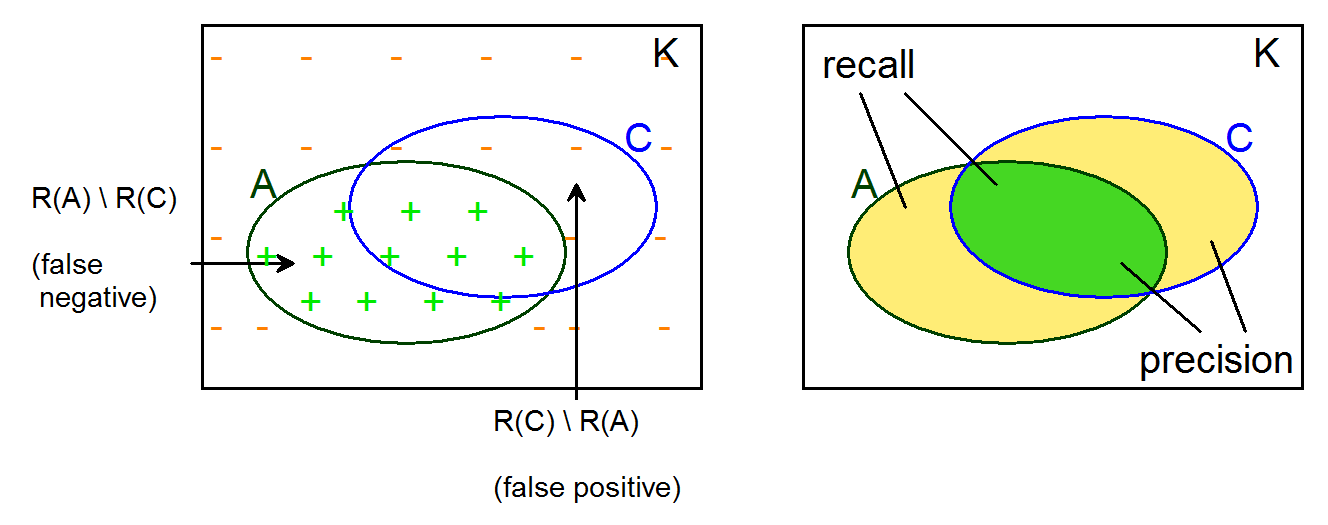
\epsfig{file=img/venn.png, width = 14 cm}
\caption{recall precision}
\end{figure*}

\section{Class Learning}
% Paper 1
\subsection*{Motivation}
The class learning approach is one method of enrichment of knowlege bases. It
aims at finding new definition of classes to extend the semantic schema. For the
motivation of the method consider the following example.

\newdef{example}{Example}
\begin{example}
For this example consider a knowlegde base containing a class \emph{President of
the United States} with instance data like Abraham Lincoln, John F. Kennedy,
Bill Clinton and Barack Obama. A class Learning algorithm may suggest that the
President class is equivalent to the following two class expressions:
\\\hspace*{12pt}\texttt{Person and born in the USA}\\
\hspace*{12pt}\texttt{American citizen and born in the USA}\footnote{The class
'American citizen' is here a subclass of 'Person', witch makes the second
statement more specific.}
\end{example}

These suggestions would then be presented to a knwolege engineer who than can
decide if they are plausible and should be added to the knowlege graph. Should
the engineer for instance choose the second statement he could check if there
are instances of the class president, where the individual is not of type
American citizen. This could indicate an error or missing information in the
knowlege graph witch could be fixed by this semi-automated approach by the
knowlege engineer.


\subsection*{Learning Problem}
The problem of learning class definitions for given data depend on the so called
inductive reasoning as opposed to inference or deductive reasoning. \cite{paper1}
Inductive Reasoning is also a key concept in Inductive Logic Programming.

\newdef{definition}{Definition}
\begin{definition}
We are searching for a formal description of the class $A$, which has existing
instances in the examined ontology. A possible class expression $C$ then
contains axioms of the form $A \subseteq C$ or $A \equiv C$.
\end{definition}

This means that the learned expression $C$ is a description of the individuals
of $A$. In our president example, the individuals are the presidents John F.
Kennedy, Barack Obama etc. whereas $C$ can be one of the suggested expression.
In many cases there will be no exact solution for $C$, but rather an
approximotion. This can be the case, if the knowlege base contains false class
assignments or missing information. In our example the birthplace of Thomas
Jefferson might be missing in the ontology. However, if most of the other
presidents have the correct birthplace the learning algorithm may still suggest
the expressions. Again, missing information may be completed by the knowlege
engineer.

In a complexe knowlege base a class learning algorithm may find many new class
definition and often different expression for the same class. Based on Occam's
razor \cite{occam-razor} simple solutions are preferred over complex ones,
because they are more readable an thus easier for the knowlege engineer to
evalueate. Simplicity is measured in an straight forward way: the lenght of an
expression, which consists of role, concept and quatifiers.
The algorithm is biased towards shorter expressions. \cite{paper1}

\subsection*{Algorithm}
One algorithm for solving the learning problem is called CELOE (Class
Expression Learning for Ontology Engineering). It is described in \cite{paper1}.
An brief overview of CELOE is given in Figure 2.
\begin{figure}
\label{celoe}
\centering
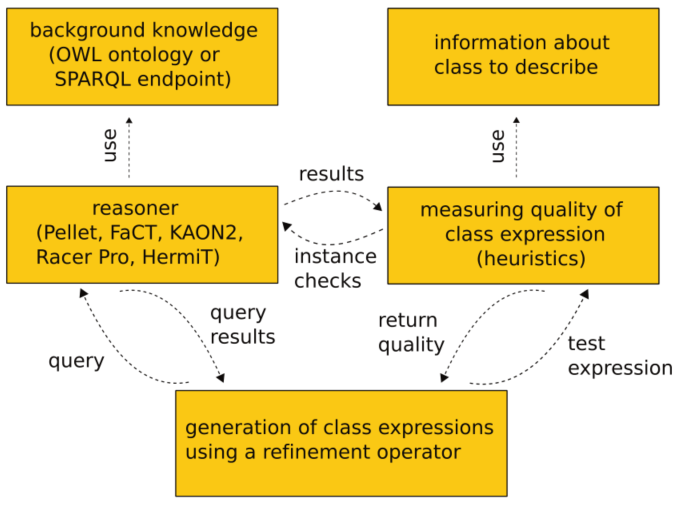
\epsfig{file=img/celoe.png, width = 8 cm}
\caption{CELOE\cite{paper1}}
\end{figure}
The algorithm follows the ``generate and test'' approach which is the common
concept in ILP. 
In the learning process many class expression are created and tested against the
background knowlege. Each of these class expressions is evalued using diffenrent
heuristics, which are described in detail in a separate section.

To find appropiate class expression to describe existing classes CELOE uses a so
called \emph{refinement operator}. The idea of these operator is based on the
work in \cite{refinement1},\cite{refinement2} and \cite{refinement3}. Refinement
operators are used to search in the space of expressions. It can be seen as a
top-downl algorithm as it is illustrated in Figure 3.
As an example consider the following path ($\leadsto$ indicates a refinement
step):\vspace{6pt}\\
$T \leadsto Person \leadsto Person \sqcap takesPartIn.T \leadsto Person \sqcap
takesPartIn.Meeting$

\begin{figure}
\label{tree}
\centering
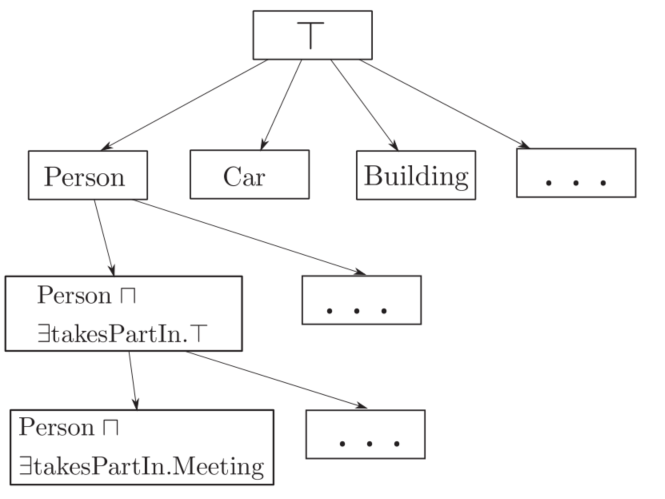
\epsfig{file=img/tree.png, width = 8 cm}
\caption{Tree\cite{paper1}}
\end{figure}

\section{Enrichment with OWL Axioms}
% Paper 2
- more

- more

- more






\section{Heuristics}
% Paper 1
\subsection{Finding the right Heuristic}
- more

- more

- more
\subsection{Efficient heuristic computation}
- more

- more

- more




\section{Evaluation Heuristics}
% Paper 1 
- more

- more

- more




\section{Evaluation on Ontology Enrichment}
% Paper 2
- more

- more

- more




\section{Related Work}

Lorem ipsum dolor sit amet, consectetur adipiscing elit. Duis luctus erat eu ex sagittis, nec cursus turpis sollicitudin. Nunc a tempor ligula. Nulla nec ante ut leo aliquam molestie vel a sapien. Quisque a imperdiet dui. Sed vehicula ipsum ornare velit ultrices, in accumsan odio placerat. Vivamus dignissim tincidunt egestas. Ut vel aliquam nisi. Vivamus vulputate justo mauris, eu interdum nunc gravida vel. Nulla suscipit odio fermentum erat efficitur dignissim. Nullam faucibus eros vel tellus aliquam luctus. Nullam quis orci eros. Aenean facilisis elit a velit posuere rutrum. 

\section{Conclusions}

Lorem ipsum dolor sit amet, consectetur adipiscing elit. Duis luctus erat eu ex sagittis, nec cursus turpis sollicitudin. Nunc a tempor ligula. Nulla nec ante ut leo aliquam molestie vel a sapien. Quisque a imperdiet dui. Sed vehicula ipsum ornare velit ultrices, in accumsan odio placerat. Vivamus dignissim tincidunt egestas. Ut vel aliquam nisi. Vivamus vulputate justo mauris, eu interdum nunc gravida vel. Nulla suscipit odio fermentum erat efficitur dignissim. Nullam faucibus eros vel tellus aliquam luctus. Nullam quis orci eros. Aenean facilisis elit a velit posuere rutrum. 


% The following two commands are all you need in the
% initial runs of your .tex file to
% produce the bibliography for the citations in your paper.
\bibliographystyle{abbrv}
\bibliography{sigproc}  % sigproc.bib is the name of the Bibliography in this case
% You must have a proper ".bib" file
%  and remember to run:
% latex bibtex latex latex
% to resolve all references
%
% ACM needs 'a single self-contained file'!

\balancecolumns
% That's all folks!
\end{document}
